
\section{Información de la asignatura}

Contenido de la asignatura:

\begin{enumerate}
\item \textbf{Preliminares} Repaso de contenidos de Cálculo II como conjuntos abiertos y cerrados, gradiente \dots
\item \textbf{Teoremas función inversa, implícita y rango} Aplicación a funciones no lineales de los teoremas fundamentales de Cálculo II
\item \textbf{Mínimos y máximos condicionados} Multiplicadores de Lagrange
\item \textbf{Subvariedades diferenciales} Objetos de dimensión n en espacios de dimensión m ($n<m$).
\item \textbf{Integración en subvariedades diferenciales} 
\item \textbf{Teorema de Stokes} Demostración del teorema con lenguaje de las formas diferenciales.
\end{enumerate}


Profesor: Jesús García Azorero, despacho 17-608, \href{mailto:jesus.azorero@uam.es}{jesus.azorero@uam.es}.

\newpage


\chapter{Preliminares}

\section{Bases del análisis matemático}

A lo largo del curso vamos a trabajar en $\real^n={(x_1,\dots c, x_n) \  x_j \in \real, j=1,...,N}$
\subsection{Producto escalar, norma y distancia}
Durante todo el año denotaremos al vector $(x_1,x_2,\dots,x_n)$ como $\gx$ por comodidad.

\begin{defn}[Producto\IS escalar euclídeo]

\[ \pesc{\gx,\gy} = \sum_{i=1}^{N} x_iy_i \]


Propiedades:
\begin{itemize}
 \item $\pesc{\lambda \gx, \gy} = \lambda \pesc{\gx, \gy}$
 \item $\pesc{\overline{x} + \overline{y}, \overline{z}}= \pesc{\gx,\gz}+\pesc{\gx,\gy}$
 \item $\pesc{gx, \gy} = \pesc{\gy,\gx}$
 \item $\pesc{\gx, \gx} ≥ 0$
 \item $\pesc{\gx,\gx} = 0 \implies \gx = \gor{0}$
\end{itemize}

Las tres primeras son la consecuencia de que el producto escalar tiene que ser bilineal.
\end{defn}

En general, un producto escalar es una matriz definida positiva y se opera de la siguiente manera:

\[\pesc{\gx,\gy} = (x_1,x_2,...,x_N) \cdot \begin{pmatrix}
a_11 &\cdots& a_1N\\ 
\vdots& \ddots & \vdots\\
a_N1 & \cdots& a_NN
\end{pmatrix}
\cdot \begin{pmatrix} y_1\\
\vdots\\ y_N \end{pmatrix}\]

 
\begin{defn}[Norma\IS euclídea]
\label{defnNorma}
\[ \md{\gx} = \left(\pesc{\gx,\gx}\right)^{\frac{1}{2}} = \dotsb = \left(\sum_{i=1}^{N}x_i^2\right)^{\frac{1}{2}} \]
Propiedades:
\begin{itemize}
 \item  $\md{\gx} = 0 \dimplies \gx = 0$
 \item	Homogeneidad: $\md{\lambda\gx} = \lambda\md{\gx}$
 \item	Desigualdad triangular: $\md{\gx+\gy} \leq \md{\gx}+\md{\gx}$
\end{itemize}
\end{defn}
\begin{lemma}
$\md{\gx} = (\gx \ast \gx) ^ \frac{1}{2}$ para cualquier producto escalar $\ast$.
\end{lemma}
\begin{defn}[Norma]
Cualquier operación que cumpla las 3 propiedades anteriores es una \textbf{norma}.

En general se tiene $\md{\cdot}_p, p \in \mathbb{N}$ y se definen todas de la misma forma:

\[ \md{\gx}_p = \left(\sum_{i=1}^N |x_i|^p \right)^\frac{1}{p} \]

\end{defn}

Hay tres casos particulares, la norma uno \index{Norma!uno}
\[ \md{\gx}_1 = |x_1| + |x_2| + ... + |x_n| \]

La norma 2, que es la norma euclídea

y la norma infinito \index{Norma!infinito}
\[\md{\gx}_{\infty} = \max\left\{|x_1|,|x_2|,\dots,|x_n|\right\} \]

 Vamos a demostrar que la norma $p$ cumple las 3 propiedades de una norma. Para ello, nos apoyaremos en dos teoremas previos:

\begin{theorem}[Desigualdad\IS de Young]
 Sea $p > 1$ y tomamos $p'$ tal que $\frac{1}{p}+\frac{1}{p'} = 1$ (exponente conjugado). Entonces:

\[ |ab| \leq \frac{1}{p} \cdot |a|^p +\frac{1}{p'} |b| ^ {p'} \]
\end{theorem}
 
\begin{proof}
Se utiliza la idea de la función logaritmo, que es cóncava\footnote{Geométricamente, cóncava significa que si uno 2 puntos de la gráfica, la recta que los une queda debajo de la gráfica.} y creciente.  Tomando 2 puntos $A$ y $B$ tenemos la condición de concavidad 

\[ t \log A + (1-t) \log B \leq \log (tA + (1-t) \cdot B)\]

Utilizando la derivada hallamos la ecuación de la recta que pasa por $A$ y por $B$ y tomamos un punto que dista $t$ de $A$ y $(1-t)$ de $B$. Como la función es cóncava sabemos que ese valor será menor que el valor del logaritmo en un punto $t$ entre $A$ y $B$.

Tomando $A=|a| ^ p$, $B = |b| ^ p$ y $t = \frac{1}{p} \rightarrow 1-t = \frac{1}{p'}$ tenemos que

\begin{align*}
\frac{1}{p}\cdot log |a|^p + \frac{1}{p'} \cdot log|b|^{p'} &\leq log\left(\frac{1}{p}|a|^p + \frac{1}{p'} |b|^{p'}\right) \\
\log \abs{a} + \log \abs{b} &\leq log\left(\frac{1}{p}|a|^p + \frac{1}{p'} |b|^{p'}\right) \\
\log \abs{ab} &\leq log\left(\frac{1}{p}|a|^p + \frac{1}{p'} |b|^{p'}\right) \\
\abs{ab} &\leq \frac{1}{p}|a|^p + \frac{1}{p'} |b|^{p'} 
\end{align*}
\end{proof} 
\begin{theorem}[Desigualdad\IS de Hölder] Se trata de una generalización de la desigualdad de Cauchy-Schwarz, que ocurre en el caso $p=2$
\[ \sum_{i=1} ^ N \abs{x_i y_i} \leq \md{\gx}_p \md{y_i}_p \]
\label{thmHolder}
\end{theorem}

\begin{proof} Tomamos  
 \begin{align*}
 a_i &= \frac{\abs{x_i}}{\md{\gx}_p} \\
 b_i &= \frac{\abs{y_i}}{\md{\gy}_{p'}}
 \end{align*}
 
 Tenemos que \[ a_i b_i \leq \frac{1}{p}a_i ^ p + \frac{1}{p'} b_i^{p'} \]
 
 Sustituimos: 
 \[  frac{\abs{x_i}}{\md{x}_{p}} \cdot \frac{\abs{y_i}}{\md{y}_{p}} \leq \frac{\abs{x_i}^p}{p\cdot \md{x}_{p}^p} + \frac{\abs{y_i}^{p'}}{p'\cdot\md{y}_{p'}^{p}} \]
 
 Tomamos sumatorios y, teniendo en cuenta que $\md{x}_{p}^p = \sum|x_i|^p$, nos queda 
 
 \[ \frac{1}{\md{x}_{p}\md{y}_{p'}}\cdot \sum_{i=1}^N |x_iy_i| \leq \frac{1}{p\md{x}_{p}^p} \sum |x_i|^p + \frac{1}{p'\md{y}_{p'}^{p'}} \sum |y_i|^{p'} = \frac{1}{p} + \frac{1}{p'} = 1 \]
 
 \end{proof}
 
Una vez probadas las dos desigualdades anteriores, pasamos a probar la desigualdad triangular: 
 
\begin{proof} El objetivo es demostrar que \[ \md{\gx+\gy}_p \leq \md{\gx}_p+\md{\gy}_p \] y vamos a hacerlo en varios pasos.
 
 Para evitarnos las raíces empezamos con $\md{\gx+\gy}_p^p$

 \begin{gather*}
 \md{\gx+\gy}_p ^ p = \sum_1 ^ N |x_i+y_i| ^ p = \sum_ 1 ^ N |x_i+y_i| \cdot |x_i+y_i| ^ {p-1} =\\
 = \sum_1 ^ N |x_i|\cdot|x_i+y_i| ^ {p-1} + \sum_1^N |y_i| \cdot |x_i+y_i|^{p-1}
 \end{gather*}

 Utilizando la desigualdad de Hölder (\ref{thmHolder}) tenemos:
 
 \begin{multline*} \md{\gx+\gy}_p ^ p \leq \\
 \sum \left(|x_i|^p\right)^{\frac{1}{p}} \cdot \underbrace{\sum \left(\left(|x_i+y_i|^{p-1}\right)^{p'}\right)^{\frac{1}{p'}}}_* +
 \sum \left(|y_i|^p\right)^{\frac{1}{p}} \cdot \underbrace{\sum \left(\left(|X_i+y_i|^{p-1}\right)^{p'}\right)^{\frac{1}{p'}}}_* 
 \end{multline*}
 
 Por ser $p$ y $p'$ exponentes conjugados es fácil comprobar que $1-\frac{1}{p'} = \frac{1}{p}$\\
 Sacamos factor común y pasamos al otro lado obteniendo (PASO INTERMEDIO?)
\[ \left(\sum_1^N |x_i+y_i|^p\right)^{\overbrace{\left(1-\frac{1}{p'}\right)}^p} = \md{\gx+\gy}_p \leq \md{x}_{p} + \md{y}_{p} \]

\textit{Guille: esta demostración es muy, muy rara.}
\end{proof}


EJERCICIO PROPUESTO: Tomamos en el plano el conjunto de los puntos cuya norma es 1. Tomando en la norma p=2 sale la circunferencia. ¿Y en p=3? 


\begin{remark} Estos argumentos se pueden utilizar para demostrar
\[ \int \abs{f\cdot g}\, dx \leq \left(\int\abs{f}^p\, dx\right) ^ \frac{1}{p} \cdot \left(\int\abs{g}^{p'}\,dx\right)^\frac{1}{p'} \]
\end{remark}

\newpage


\begin{defn}[Distancia\IS euclídea]
\[d(\gx,\gy) = \md{\gy - \gx} \]
\end{defn}

Propiedades:
\begin{itemize}
 \item La distancia es siempre positiva: $d(\gx,\gy)\ge 0$
 \item $d(\gx,\gx) = 0$
 \item Simetría: $d(\gx,\gy) = d(\gy, \gx)$
 \item Desigualdad triangular $d(\gx,\gz) \leq d(\gx,\gy) + d(\gy,\gz)$. La distancia entre 2 puntos es menor o igual en línea recta que pasando por un punto intermedio.
\end{itemize}


\begin{defn}[Distancia] Cualquier operacion que cumpla las 3 propiedades anteriores es una distancia. \end{defn}

\paragraph{Recapitulando}
Con un producto escalar puedo definir una norma y con esa norma puedo definir una distancia. Pero... ¿Podemos definir una norma 
que no venga de un producto escalar y/o alguna distancia que no provenga de una norma? Sí, por ejemplo

\[ \tilde{d} (\gx,\gy) = \abs{\arctg(y) - \arctg(x)} \] 

No cuesta mucho comprobar que cumple las 3 propiedades de una distancia. Además, esta distancia es cuanto menos curiosa porque nunca será mayor de $\pi$.

 Podemos comprobar que si existiera una norma que midiese esta distancia tendríamos \[\tilde{\md{\gx}} = \tilde{d} (\gx,\gor{0}) = \abs{\arctg (x)} \]
 pero esto no cumple la propiedad: $\tilde{\md{\lambda x}} = \abs{\arctg \lambda x} \neq \abs{\lambda}\abs{\arctg x} = 
 \abs{\lambda x}\tilde{||x||}$
 ya que ninguna distancia puede ser mayor que $\pi$ y tomando un $\lambda > \pi$ se produciría la contradicción.

\subsubsection{Relación norma - producto escalar}
\label{secNormaprodEsc}
\begin{theorem}
Supongamos que tengo un producto escalar $\ast$ y una norma asociada \[ \md{\gx} = (\gx\ast \gx) ^ {\frac{1}{2}}\]. Entonces \[ \md{\gx + \gy}^ 2 =  \md{\gx} ^ 2 + \md{\gy} ^ 2+2(\gx\ast\gy) \]
\end{theorem}

\begin{proof}
\[ \md{\gx+\gy}^2 = (\gx+\gy)\ast(\gx+\gy) = \gx \ast \gx + \gx \ast \gy + \gy \ast \gx + \gy \ast \gy=\md{\gx} ^ 2 + \md{\gy} ^ 2+2(\gx\ast\gy) \]
\end{proof}

Esa norma asociada al producto escalar tiene dos propiedades importantes:
\begin{itemize}
\item Paralelogramo: $\md{\gx+\gy}^ 2 + \md{\gx-\gy} ^ 2 = 2\left(\md{x}^2+\md{y}^2\right) $
\item Polarización: $\md{\gx+\gy} ^ 2 - \md{\gx-\gy} ^ 2 = 4(\gx*\gy)$
\end{itemize}


\subsubsection{Equivalencia de normas}
Sea $\md{\cdot}$ una norma en $\real^N$. Si intento calcular la norma de un vector $\gx$

\[ \md{\gx} = \md{\sum x_i e_i} \leq \sum_{i=1}^N \md{x_1 e_1} = \sum_{i=1}^N|x_i|\cdot\md{e_i} \]

Tenemos: $\md{\gx} \leq \sum_{i=1}^N c_i |x_i|$ siendo $c_i = \md{e_i}$. Aplicando Cauchy-Schwarz  nos queda
\[ \sum_{i=1}^N \left(c_i^2\right)^\frac{1}{2} \cdot \sum \left(|x_i|^2\right)^\frac{1}{2} \]
Es decir, puedo controlar cualquier norma con una constante y la norma euclídea:
$$|||\gx||| \leq C \md{x}_{2}$$
En particular, $0 \leq |||\gor{x_n} - \gx|||\leq c ||\gor{x_n}-\gx||$. 

\begin{remark}
Si aplicamos Holder en vez de Cauchy, sale la igualdad con la norma p y no con la euclídea.
\end{remark}

\paragraph{Aplicación:}
Sea $F(\gx) = |||\gx|||$ y $F:\real^N \rightarrow \real^N$ 
$$|F(\gx)-F(\gy)| = \left| |||\gx - \gy||| \right| = |||\gx - \gy||| \leq C ||\gx - \gy||$$
Utilizando: $|||\ga-\gb||| \ge |||\ga||| - |||\gb|||$ \footnote{(la desigualdad triangular con restas, que se saca con un simple cambio de variable)}

Es decir, cualquier norma en $\real^n$ es \textbf{continua} respecto de la norma euclídea. \footnote{Continua si la tomas como una función de $\real^N$ en $\real$}

\begin{theorem}[Relación norma $\leftrightarrow$ producto escalar]
$\md{\cdot}$ una norma cualquiera de $\real^N$ proviene de un producto escalar si y sólo si la norma satisface la identidad del paralelogramo. 
\end{theorem}

\begin{proof}
En el apartado anterior (\ref{secNormaprodEsc}) demostramos la implicación hacia la derecha. Vamos a demostrar la recíproca:
Suponemos que la norma satisface la identidad del paralelogramo:

\begin{equation}
 \md{\ga+\gb}^2 + \md{\ga-\gb}^2 = 2 \md{\ga}^2 + 2\md{\gb}^2 \label{eqParalelogramo}
\end{equation}
Queremos probar que existe un producto escalar $\ast$ tal que $\md{\gx} = (\gx\ast \gx)^\frac{1}{2}$, así que definimos uno utilizando la identidad de polarización: 

\begin{equation}
 \gx\ast\gy = \frac{1}{4} \left( \md{\gx+\gy} ^ 2 - \md{\gx-\gy} ^ 2\right) \label{eqPolarizacion}
 \end{equation}

Queremos probar que, efectivamente, $\ast$ es un producto escalar, así que tenemos que demostrar las siguientes propiedades:
\begin{enumerate}
 \item $\gx\ast\gy = \gy\ast\gx$ .
 \item $\gx\ast\gx \ge 0\quad \forall\; \gx$
 \item $(\gx\ast\gx) = 0 \dimplies \gx=\gor{0}$ 
 \item $(\lambda \gx) \ast \gy = \lambda\left(\gx\ast\gy\right)$
 \item $(\gx+\gy)\ast\gz =\gx\ast\gx + \gy\ast\gz $
\end{enumerate}

Las propiedades 1, 2 y 3 son triviales. Vamos con 4 y 5

\paragraph{Demostración de la 4ª propiedad}

Demostraremos que se cumple por inducción cuando $\lambda\in\nat$. Primero probamos para $\lambda = 2$.

\begin{align*}
(2\gx)\ast\gy = && \text{usando (\ref{eqPolarizacion})} \\
= \frac{1}{4} \left(|||2\gx+\gy |||^2 - |||2\gx-\gy |||^2\right) = && \\
= \frac{1}{4} \left(|||\underbrace{\gx}_a + \underbrace{\gx+\gy}_b|||^2 - |||\underbrace{\gx}_a+\underbrace{\gx-\gy}_{-b}|||^2\right) = && \text{usando (\ref{eqParalelogramo})} \\
= \frac{1}{4} \left(2|||\gx|||^2 + 2|||\gx + \gy|||^2\right) = && \\
= 2 \frac{1}{4} \left(|||\gx+\gy|||^2 - |||\gx-\gy|||^2\right) = 2 (\gx\ast\gy) &&
\end{align*}

Conclusión: si $\lambda = 2$ vemos que sale fuera y por lo tanto se cumple.

Paso 2 de la inducción: buscamos demostrar la propiedad con $\lambda = n$ con $n \in \mathbb{N}$

\begin{align*}
(n\gx)\ast\gy = && \text{usando (\ref{eqPolarizacion})} \\
= \frac{1}{4} \left(|||n\gx+\gy|||^2 - |||n\gx-\gy|||^2\right) = && \\
= \frac{1}{4} \left(|||\underbrace{(n-1)\gx}_a+\underbrace{\gx+\gy}_b|||^2 
		- ||| \underbrace{(n-1)\gx}_a+ \underbrace{\gx-\gy}_b|||^2\right)= && \text{usando (\ref{eqParalelogramo})} \\
=...=2(\gx\ast\gy) + (n-2)(\gx\ast\gy) = && \text{usando hip. de inducción}\\
= n (\gx\ast\gy)
\end{align*}

Queda demostrado por lo tanto para $\lambda \in \nat$. Falta ahora demostrarlo para el resto de conjuntos de números.

\textbf{Para $\lambda \in \ent$} utilizaremos $(-\gx) \ast \gy = - (\gx\ast\gy)$ y podremos usar la demostración de los naturales.

\textbf{Para $\lambda = n \in \rac$} con $n = \frac{p}{q}$, siendo $p$ y $q$ primos entre sí, vemos que 

\[ \left(\frac{p}{q}\gx\right)\ast\gy = \frac{q\left(\left(\frac{p}{q}\gx\right)\ast\gy\right)}{q} = \frac{\left(q\cdot\frac{p}{q}\gx\right)\ast\gy}{q} = \frac{\left(p\gx\ast\gy\right)}{q} \] que tal y como habíamos demostrado antes es igual a $ \dfrac{p\left(\gx\ast\gy\right)}{q} $, con lo que queda demostrado también para los racionales.

Por último, queremos demostrarlo cuando $\lambda \in \real$

$\lambda = \liminf{n} r_n$. Utilizaremos el resultado previo de que cualquier norma es continua.

$\gx, \gy$ fijos.

Revisar: Los $|||r_n \gx + \gy|||^2$ y  $|||r_n \gx - \gy|||^2$ son continuos.
$$\alpha \gx*\gy = \frac{1}{4}\left(||r_n \gx + \gy|||^2||| -|||r_n \gx - \gy|||^2||| \right) =$$
$$\lim_{n\to\infty} \left(||r_n \gx + \gy|||^2||| -|||r_n \gx - \gy|||^2||| \right) = \lim_{n\to\infty} (r_n\gx*\gy) = $$
$$\lim_{n\to\infty} r_n(\gx*\gy) = \alpha (\gx*\gy)$$

WTF es esto.

\paragraph{Demostración de la 5 propiedad:}
$$A = (\gx+\gy)*\gz = \frac{1}{4} \left( |||\gx+\gy+\gz|||^2 - |||\gx+\gy-\gz|||^2\right)$$
$$B =\gx*\gz = \frac{1}{4} \left( |||\gx+\gz|||^2 - |||\gx-\gz|||^2\right)$$
$$C =\gy*\gz = \frac{1}{4} \left( |||\gy+\gz|||^2 - |||\gy-\gz|||^2\right)$$
Demostraremos que $A-B-C=0$\\
COMPLETAR la comprobación.
\end{proof}

\begin{remark}
$d(\gx,\gy) = |||\gx-\gy||| \text{ para alguna norma }|||\cdot||| \dimplies (d(\gx+\gz)+d(\gy+\gz) = d(\gx,\gy) \wedge d(\lambda \gx,\lambda \gy = \abs{\lambda} d(\gx,\gy))$
\end{remark}

\subsection{Topología}
\begin{defn}[Bola] Se define la bola de radio $R$ centrada en el punto $\gx_0$ como 
\[B_R(\gx_0) =\{\gx \in \real^N \tq \underbrace{d(\gx,\gx_0)}_{=\md{\gx-\gx_0}} < R \} \]
\end{defn}


Para evitar jaleos, al tratar la distancia vamos a tomar la norma euclídea. Como todas las normas son equivalentes, nos da igual tomar una que otra.
\begin{defn}[Conjunto\IS abierto] Un conjunto $A \subset \real^N$ es abierto si y sólo si $\forall\, \ga\in A\; \exists \varepsilon > 0 \tq B_\varepsilon(\ga) \subset A$
\end{defn}

\begin{defn}[Conjunto\IS cerrado] Un conjunto $B \subset \real^N$ es cerrado si y sólo si su complementario $B^c= \real^N-B$ es abierto.
\end{defn}

\begin{theorem}[Caracterización de cerrados en términos de sucesiones][Caracterización!por cerrados]\label{thmCerradoSucesiones} Un conjunto $B \subset \real^N$ es cerrado si y sólo si para cualquier sucesión convergente $\{x_n\} \subset B$ se cumple que  $\lim x_n \in B$. 
\end{theorem}

\begin{theorem}[Operaciones con conjuntos abiertos y cerrados][]
Suponemos conjuntos de dimensión finita:
\begin{itemize}
 \item Unión arbitraria de abiertos $\rightarrow$ abierto
 \item Intersección finita de abiertos $\rightarrow$ abierto
 \item Union finita de cerrados $\rightarrow$ cerrado
 \item Intersección arbitraria de cerrados $\rightarrow$ cerrado
\end{itemize} 
\end{theorem}

\begin{defn}[Punto\IS de acumulación]\label{defPtoAcc}
La idea intuitiva es aquellos puntos a los que puedo llegar en el límite, es decir, puntos que a su alrededor a una distancia arbitrariamente pequeña existen otros puntos del conjunto.
\[ A\subset \real^N,\; a \in (A) \dimplies  \forall \varepsilon > 0\; (B_{\varepsilon} (a) \setminus \{a\}) \cap A \neq \emptyset \]
Siendo $(A)$ es el conjunto de los puntos de acumulación.
\end{defn}

\begin{defn}[Frontera]
La frontera $∂A$ de un conjunto $A$ son aquellos puntos para los que en su entorno (para cualquier $\varepsilon$) hay puntos tanto del conjunto como puntos de fuera del conjunto.
\[ a \in ∂A \dimplies \forall \varepsilon>0 \tq B_\varepsilon (a) \cap A \neq \emptyset \y B_{\varepsilon} (a) \cap A^C \neq \emptyset \]
\end{defn}

\begin{defn}[Interior] El interior es el conjunto abierto más grande que está contenido en el conjunto $A$.\end{defn}
\begin{defn}[Cierre]\label{dfnCierre} El cierre de un conjunto $A$ es el conjunto cerrado más pequeño en el que está contenido $A$.\end{defn}

\begin{remark}
Cierre e interior no los vamos a definir formalmente porque se dan por supuesto.
\end{remark}

\begin{defn}[Conjunto\IS compacto]
\label{defCompacto}
Un conjunto que cumpla cualquiera de las 3 propiedades siguientes.
\end{defn}

\begin{theorem}[Conjunto\IS cerrado y acotado]\label{thmCerradoAcotado}
Sea $K \subset \real^N$. Son equivalentes:
\begin{enumerate}
 \item \label{propCerrado} K cerrado y acotado.
 \item \label{propSucesion} Para cualquier sucesión $\{x_n\} \subset K$, podemos encontrar una subsucesión convergente $\{x_{n_j}\} \subset\{x_n\}$ con $\lim x_{n_j} \in K$.
 \item \label{propRecubrimiento} Dado cualquier recubrimiento $\{A_i\}$ abierto de modo que $K \subset \cup \{A_i\}$ puedo encontrar un recubrimiento finito $\{A_j\}, j=1,...,M \tq K \subset \bigcup_{i=1}^M A_i$
\end{enumerate}
\end{theorem}

\begin{proof}

\paragraph{2 implica 1}  Supongamos que $K$ no estuviera acotado (negamos la propiedad \ref{propCerrado}). Consideremos una sucesión de vectores $\{x_n\}$ de tal forma que $\md{x_n} = n$, creciente y no acotada, pero con todos los elementos en $K$. Es imposible encontrar una subsucesión convergente, lo que contradice \ref{propSucesion}.

Si, por otra parte, $K$ no fuera cerrado, tendríamos que la frontera está fuera del conjunto, y podemos encontrar una sucesión $\{x_n\}$ con $\lim x_n \in ∂K$, lo que contradice \ref{propSucesion}.

\paragraph{1 implica 2} Empecemos por el caso sencillo, explorando una sucesión cualquiera $\{\gx_n\} \subset K \subset \real$, donde $K$ es, como decíamos en el enunciado, cerrado y acotado. Para encontrar una subsucesión convergente, usaremos el criterio de bisección.

\begin{center}
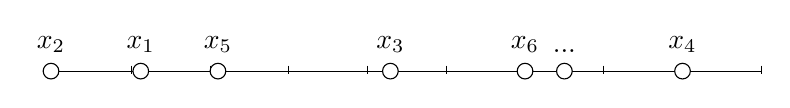
\begin{tikzpicture}
% a straight line segment
\draw (1,0) -- (10,0);
\foreach \x  in {1,...,10}
  \draw[xshift=\x cm] (0pt,2pt) -- (0pt,-1pt);
% the labels
\node[fill=white,draw=black,circle,inner sep=2pt,label=above:{$x_1$}] at (2.12,0) {};
\node[fill=white,draw=black,circle,inner sep=2pt,label=above:{$x_2$}] at (0.98,0) {};
\node[fill=white,draw=black,circle,inner sep=2pt,label=above:{$x_3$}] at (5.29,0) {};
\node[fill=white,draw=black,circle,inner sep=2pt,label=above:{$x_4$}] at (9,0) {};
\node[fill=white,draw=black,circle,inner sep=2pt,label=above:{$x_5$}] at (3.1,0) {};
\node[fill=white,draw=black,circle,inner sep=2pt,label=above:{$x_6$}] at (7,0) {};
\node[fill=white,draw=black,circle,inner sep=2pt,label=above:{...}] at (7.5,0) {};
\end{tikzpicture}
\end{center}

Escogemos el primer elemento $g_1$ de nuestra subsubcesión, y dividimos por la mitad el segmento.

\begin{center}
\begin{tikzpicture}
\draw (1,0) -- (10,0);
\foreach \x  in {1,...,10}
  \draw[xshift=\x cm] (0pt,2pt) -- (0pt,-1pt);
% the labels
\node[fill=black,draw=black,circle,inner sep=2pt,label=above:{$x_1$},label=below:{$g_1$}] at (2.12,0) {};
\node[fill=white,draw=black,circle,inner sep=2pt,label=above:{$x_2$}] at (0.98,0) {};
\node[fill=white,draw=black,circle,inner sep=2pt,label=above:{$x_3$}] at (5.29,0) {};
\node[fill=white,draw=black,circle,inner sep=2pt,label=above:{$x_4$}] at (9,0) {};
\node[fill=white,draw=black,circle,inner sep=2pt,label=above:{$x_5$}] at (3.1,0) {};
\node[fill=white,draw=black,circle,inner sep=2pt,label=above:{$x_6$}] at (7,0) {};
\node[fill=white,draw=black,circle,inner sep=2pt,label=above:{...}] at (7.5,0) {};

\draw[draw=red,ultra thick] (5.5,-1) -- (5.5,1);
\node[text=red] at (5.5,-1.3) {1};
\end{tikzpicture}
\end{center}

En al menos una de las dos mitades del segmento habrá infinitos términos: cogemos esa mitad y repetimos los mismos pasos. Finalmente, llegaremos a una subsucesión de este estilo:

\begin{center}
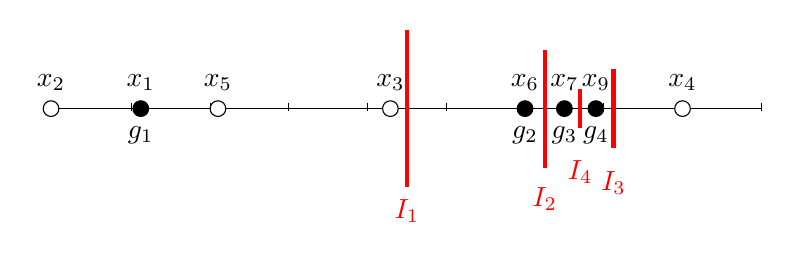
\begin{tikzpicture}
\draw (1,0) -- (10,0);
\foreach \x  in {1,...,10}
  \draw[xshift=\x cm] (0pt,2pt) -- (0pt,-1pt);
% the labels
\node[fill=black,draw=black,circle,inner sep=2pt,label=above:{$x_1$},label=below:{$g_1$}] at (2.12,0) {};
\node[fill=white,draw=black,circle,inner sep=2pt,label=above:{$x_2$}] at (0.98,0) {};
\node[fill=white,draw=black,circle,inner sep=2pt,label=above:{$x_3$}] at (5.29,0) {};
\node[fill=white,draw=black,circle,inner sep=2pt,label=above:{$x_4$}] at (9,0) {};
\node[fill=white,draw=black,circle,inner sep=2pt,label=above:{$x_5$}] at (3.1,0) {};
\node[fill=black,draw=black,circle,inner sep=2pt,label=above:{$x_6$},label=below:{$g_2$}] at (7,0) {};
\node[fill=black,draw=black,circle,inner sep=2pt,label=above:{$x_7$},label=below:{$g_3$}] at (7.5,0) {};
\node[fill=black,draw=black,circle,inner sep=2pt,label=above:{$x_9$},label=below:{$g_4$}] at (7.9,0) {};
\draw[draw=red,ultra thick] (5.5,-1) -- (5.5,1);
\node[text=red] at (5.5,-1.3) {$I_1$};

\draw[draw=red,ultra thick] (7.25,-0.75) -- (7.25,0.75);
\node[text=red] at (7.25,-1.15) {$I_2$};

\draw[draw=red,ultra thick] (8.125,-0.5) -- (8.125,0.5);
\node[text=red] at (8.125,-0.95) {$I_3$};

\draw[draw=red,ultra thick] (7.7,-0.25) -- (7.7,0.25);
\node[text=red] at (7.7,-0.8) {$I_4$};
\end{tikzpicture}
\end{center}

Nuestra subsucesión $\{g_x\}$ es igualmente infinita. Tal y como la hemos definido, tenemos que cada $g_i$ está en un intervalo $(I_i, I_{i-1})$ que cada vez se hace más pequeño. Es decir, que la subsucesión $\{g_x\}$ es de Cauchy y, por lo tanto convergente.

Ahora sólo queda ver cómo podríamos obtener esa subsucesión cuando estamos en espacios que no sean $\real^N$. La idea es sencilla: primero, buscamos una subsucesión que converja en la primera coordenada. Dentro de esa subsucesión, buscamos otra subsucesión que converja además en la segunda, y así con las $N$ coordenadas. 
\end{proof}

\begin{theorem} \label{thmCompactoMax} Sea $K\subset \real$ un conjunto compacto. Entonces, si $\appl{f}{\real}{\real}$ es continua en $K$ existen  $x_m,x_M \in K \tq F(x_m) \leq F(x) \leq F(x_M)\;\forall x \in K$.

Es decir, si $F$ es continua en $K$ alcanza su máximo y su mínimo en el conjunto.
\end{theorem}

\paragraph{Aplicación:}
$F(\gor{x}) = |||\gor{x}|||$ una norma (que ya sabemos que es continua):

\emph{Conclusión:} $m \md{x} \leq |||\gor{x}||| \leq C||\gor{x}||$

\begin{theorem}
En $\real^N$ TODAS las normas son equivalentes. 
\end{theorem}

\subsubsection{Conexión}
\begin{defn}[Conexión\IS por caminos]
Dados $a,b \in C$ podemos encontrar una aplicación continua $\appl{\varphi}{[0,1]}{\real^N}$ tal que $\varphi(0) = a$ y  $\varphi(1) = b$ con $ \varphi(t) \in C\, \forall t \in [0,1]$. 

Es decir, $C$ es conexo por caminos si podemos encontrar una "línea", un camino que una dos puntos cualquiera del conjunto y que además no se salga del conjunto.
\end{defn}

\begin{defn}[Conexión\IS por abiertos]
$C$ es conexo por conjuntos si para cualquier par de abiertos $A,B \subset \real^N \tq C\subset A\cup B$ se cumple que, si $A\cap C\neq \emptyset \y B\cap C \neq \emptyset $ entonces $ A\cap B \neq \emptyset$.

Esto es equivalente a decir que $C$ no puede ser expresado como unión de dos conjuntos disjuntos.
\end{defn}


\begin{remark}

\begin{figure}[hbtp]
\label{imgPeine}
\begin{center}
\begin{tikzpicture}

\draw (1,0) -- (10,0);

\foreach \x  in {2,...,20}
  \draw ($10/\x*(1,0) + (0.49,0)$) -- ($(0.49,3) + 10/\x*(1,0)$);

\node[fill=white,draw=black,circle,inner sep=2pt] at (1,0) {};

\end{tikzpicture}
\caption{Conjunto peine}
\end{center}
\end{figure}

Es curioso comprobar que estas 2 definiciones no son equivalentes. Tomemos el conjunto peine (figura \ref{imgPeine})
\[ \left\{(x,0), x\in (0,1]\right\} \cup \{(0,y), y \in (0,1]\} \cup \left\{\bigcup_{n=1}^{\infty}{\left(\frac{1}{n},y\right), y \in [0,1]}\right\} \]

Es un conjunto conexo por abiertos porque no podemos separarlo en dos conjuntos disjuntos. Sin embargo, no es conexo por caminos porque, si queremos ir del punto $(0,1)$ al $(0,0.5)$ no podemos hacerlo ya que el único camino pasaría por el punto $(0,0)$, que no está en el conjunto.
\end{remark}

\subsection{Funciones continuas, abiertos y cerrados}
 
 Al tener definida una norma de vectores podemos definir convergencia y continuidad:

\begin{defn}[Convergencia] Se dice que $\gx_n$ converge a $\gx$ (notación: $\gx_n \to \gx$) si

\[  \forall \varepsilon > 0\; \exists n_0 \tq n > n_0 \implies \md{\gx-\gor{x}_n}<\varepsilon \]

\end{defn}

\begin{defn}[Función\IS continua] Sea $\appl{F}{\real^N}{\real^M}$. Se dice que $F$ es continua en $a$ si y sólo si 

\[  \forall \varepsilon > 0 , \exists \delta > 0 \tq \md{\gx-\ga}_a < \delta \Rightarrow \md{F(\gx)-F(\ga)}_b< \varepsilon \]
\label{dfnContinua}
\end{defn}

\begin{remark} Es interesante ver que se puede hablar de continuidad tomando una norma en $\mathbb{R}^N$ y otra distinta en $\real^M$ sin por ello variar la definición de continuidad, teniendo en cuenta que todas las normas son equivalentes. \end{remark}

A partir de esta definición podemos estudiar qué hacen las funciones continuas con conjuntos abiertos y cerrados. Sea $F$ continua. Contrario a lo que podríamos intuir, 

\begin{enumerate}
\item A abierto no implica que  $F(A)$ sea abierto.
\item B cerrado no implica que $F(B)$ sea cerrado.
\end{enumerate}

Empezamos definiendo en qué consiste una función inversa:

\begin{defn}[Función\IS inversa] Dada \[\appl{F}{\real^N}{\real^N}\], definimos su inversa como
\[ \inv{F}(A) = \left\{\gor{x}\in \real^N \tq F(\gor{x})\in A\right\} \]
\end{defn}

A partir de aquí podemos extraer dos conclusiones que sí nos ayudarán a discernir si un conjunto imagen es abierto y cerrado.

\begin{theorem}[Función\IS inversa]\par\noindent\par
\label{thmInversa}
\begin{itemize}
\item F continua y A abierto $\implies F^{-1} (A)$ abierto.
\item F continua y B cerrado $\implies F^{-1} (A)$ cerrado.
\end{itemize}
\end{theorem}

Este teorema nos sirve para decir fácilmente si un conjunto es abierto o cerrado. Por ejemplo, consideremos
 \[ M=\{(x,y,z) \in \real^3 \tq x^2 + \cos\left(x\abs{y}\right) - e^z < 1 \} \]

Podemos definir ahí la función $F$ como 
\[ F(x,y,z) = x^2 + \cos\left(x\abs{y}\right) - e^z\]

que va de $\real^3$ a cierto conjunto $A = \{ a \in \real \tq a < 1 \}$. Podemos reescribir $M$ como
\[M=\{(x,y,z) \in \real^3 \tq  F(x,y,z) \in A\}\]

o, de otra forma, $M = \inv{F}(A)$. Según el teorema (\ref{thmInversa}), como $A$ es abierto entonces $M$ también es abierto.

\begin{proof} Demostramos las dos implicaciones que hemos enunciado.

1) Dado un $\gor{x} \in F^{-1} (A)$ queremos hallar un $R>0$ tal que $B_R(\gor{x})\subset F^{-1} (A)$. Partimos de 
\[\gor{x}\in F^{-1} (A) \dimplies F(\gor{x})\in A\]

Como $F$ es continua, $\exists \varepsilon>0 \tq B_{\varepsilon}(F(\gor{x}))\subset A$. Esto es equivalente a decir que, para cualquier $\gz$
\[ ||\gor{z}-F(\gor{x})|| < \varepsilon \implies \gor{z}\in A\]

Por la definición de continuidad (\ref{dfnContinua}), dado un $\gor{s}\in B_R(\gor{x})$ 

\[ \exists \delta > 0 \tq ||\gor{x}-\gor{s}||<\delta \implies ||F(\gor{x})-F(\gor{s})||< \varepsilon \]


y por lo tanto $F(\gor{s}) \in A$ y $\gor{s} \in F^{-1} (A)$.
Conclusión: Hemos encontrado un $\delta > 0$ tal que $s \in B_R(\gor{x}) \implies s \in F^{-1} (A)$.
\end{proof}

\section{Aplicaciones lineales y matrices}

\subsection{Aplicaciones lineales}

\begin{defn}[Aplicación\IS lineal]

Sea: $\appl{L}{\real^N}{\real^M}$. Entonces, $L$ es lineal si y sólo si

\[ L(\lambda \gor{x}) = \lambda L(\gor{x}) \] 
\[ L(\gor{x}+\gor{y}) = L(\gx)+L(\gy)\] 

\end{defn}
Además, toda aplicación lineal se puede escribir en forma de matriz.

\[L(\gor{x})=A\gor{x} =
\begin{pmatrix}
a_{11} 	& \cdots & a_{1n}		\\
\vdots	& \ddots &  \vdots 	\\
a_{n1}	& \cdots & a_{nn} 
\end{pmatrix}\]

\begin{theorem}
Toda aplicación lineal $L$ es continua.
\end{theorem}
\begin{proof} Partiendo de la definición de continuidad (\ref{dfnContinua}), $L$ es continua si y sólo si

\[ \forall \ga, \gx \; \forall \epsilon > 0 \; \exists \delta > 0 \tq \md{\ga - \gx} < \delta \implies \md{L\ga - L\gx} < \epsilon \]

Sabemos que $\md{A\gx} ≤ C\md{\gx}$ para alguna constante $C$. Podemos reescribir

\[ \md{L\ga - L\gx} = \md{L(\ga-\gx)} ≤ C\md{\ga-\gx} \]

Entonces, la igualdad se cumple si tomamos $\epsilon = C\delta$.
\end{proof}

\subsection{Norma de matrices}
Consideramos una aplicación continua

\begin{align*}
\appl{F}{\real^N&}{\real} \\
\gor{x} &\longrightarrow F(\gx) = \underbrace{||A\gx||}_{L(\gx)}
\end{align*}

Sabemos que existe $C>0$ tal que $||A\gx|| \leq C||\gx||$, es decir,  $||A\gx||\leq C$ si $||\gx||=1$. Queremos saber cuál es la mejor constante que podemos encontrar, la que más se ajuste. Consideramos el conjunto $M$ de todos los vectores de la esfera unidad, es decir 

\[ M = \{||A\gx|| \tq ||\gx||=1\}\subset \real \]

Entonces mejor constante $C$ es la cota superior mínima (supremo) que vamos a llamar $\alpha$. Al ser $F$ continua y $M$ compacto, sabemos que el supremo $\alpha \in M$.

\begin{defn}[Norma\IS de una matriz]
$$\norm{A} = \alpha = \max{\norm{A\gx} \tq \norm{\gx} =1}$$
\end{defn}

\begin{proof} Hay que demostrar que esta norma que hemos definido cumple las propiedades de una norma (\ref{defnNorma}). Las dos primeras son triviales, demostremos la desigualdad triangular
\[ \norm{A+B} = \max{\norm{(A+B)\gx}} = \norm{(A+B)\gx_{A,B}} \] 

donde $\gx_{A,B}$ es el vector que da el valor máximo para esa multiplicación. Usando la propiedad asociativa

\[  \norm{(A+B)\gx_{A,B}} = \norm{A\gx_{AB} + B\gx_{A,B}} ≤ \norm{A\gx_{A,B}} + \norm{B\gx_{A,B}} \]

Sabemos que existen dos vectores $\gx_A$ y $\gx_B$ que maximizan el resultado $\norm{A\gx_A}$ y $\norm{A\gx_B}$ respectivamente, por lo tanto

\[ \norm{A\gx_{A,B}} + \norm{B\gx_{A,B}} ≤ \norm{A\gx_A} + \norm{B\gx_B} = \norm{A} + \norm{B} \]

\end{proof}

Basándonos en lo que hemos obtenido, calculamos la norma uno de 
\[A = \begin{pmatrix}
      1&2\\-3&1\\2&0
     \end{pmatrix}\]  

Tenemos que maximizar, sabiendo que $|x|+|y| = 1$:

\[ |x+2y| + |-3x+y| + |2x| \leq |x|+|2y| + |3x| + |y| + 2|x| = 6|x|+3|y| \leq 6 (|x|+|y|) =6 \]
¿Podemos encontrar un vector $\gx = (x_0,y_0)$ tal que $||A(x_0,y_0)^T||_1 = 6$?\\
Tomando $x_0 = 1$ y $y_0 = 0$ lo encontramos. Como $\gx$ está en la esfera unidad y es una cota, es el máximo y por lo tanto la norma que buscamos.

Curiosamente, \textbf{coincide con la suma de los valores absolutos de las columnas} y escoger el más grande.

Si tomamos la norma infinito de 
\[A = \begin{pmatrix}
      1&2\\-3&1\\2&0
     \end{pmatrix}\]

Tenemos que \textbf{coincide con el máximo de las posibles sumas de los valores absolutos de las filas}.



Queremos buscar ahora cuánto vale la norma de una matriz cuando usamos la norma euclídea. Usaremos los dos lemas siguientes para apoyarnos.

\begin{lemma}
 Sea A una matriz cualquiera, entonces $\trans{A}A$ es simétrica.
\end{lemma}
\begin{lemma}
 \[ \underbrace{\pesc{\gx,A\gy}}_{\text{Producto en } \real^n} = \underbrace{\pesc{A^T \gx,\gy}}_{\text{Producto en } \real^M} \]
\end{lemma}

Tenemos $A^TA$ diagonalizable, de dimensión $N \times N$. Buscamos cuánto vale $\norm{A\gx}$ con  $\gx \in \real^N$. Empezamos desarrollando el vector en una base ortonormal de  $A^T A$: \[ \gx = \sum \alpha_i \gv_i \] y por lo tanto \[ ||\gx|| = \sum \alpha_i^2 \pesc{\gv_i,\gv_i}\].
 
 Desarrollamos el producto \[\trans{A}A\gx = \trans{A}A\left(\sum \alpha_i \gv_i\right) = \sum \left(\alpha_i\lambda_i\gor{v}_i\right) \] donde $\lambda_i$ son los autovalores de $\trans{A}A$. 
 
 Ahora queremos hallar el máximo de $||A\gx||$ cuando $||\gx|| = 1$:
 
 \[ ||A\gx||^2 = \pesc{A\gx,A\gx} = \pesc{\trans{A}A\gx,\gx} = \pesc{\sum \lambda_i \alpha_i \gv_i,\sum\alpha_i \gv_i} \]
 
 Como la base de $\{\gv_n\}$ es ortonormal, $\pesc{\gv_i, \gv_j} = 0$ si $i≠j$, por lo tanto sólo nos queda
 \[ \pesc{\sum \lambda_i \alpha_i \gv_i,\sum\alpha_i \gv_i} = \sum \lambda_i \alpha_i^2 \leq \lambda_{max} \left(\sum \alpha_i^2\right) = \lambda_{max} \]
 
 teniendo en cuenta que $\norm{\gx} = 1$ y donde $\lambda_max$ es el autovalor máximo. Es decir, hemos llegado a que
 \[ \max\norm{A\gx} ≤ \sqrt{\lambda_{max}} \]
 
 Hemos definido una cota para $\norm{A\gx}$. Ahora bien, esa cota se alcanza cuando $\gx$ es el autovector asociado a $\lambda_{max}$, por lo tanto la cota es un máximo y la norma de la matriz.
 
 \section{Límites}
 
 \begin{defn}[Límite] Dada una función $\appl{F}{\real^N}{\real^M}$, definimos su límite cuando $\gx\to\ga$ de la siguiente forma:
  \[ \lim_{\gx \rightarrow \ga} F(\gx) = \gor{L} \dimplies \forall \varepsilon > 0,  \exists \delta>0 \tlq 0<||\gx-\ga|| <\delta \implies ||F(\gx) - L||<\varepsilon\] 
 \end{defn}
 
 Importante el detalle de $0 < ||\gx-\ga||$, no es un $\leq$, porque no se necesita que la función esté siquiera definida en el punto $\ga$.  
 
 \begin{theorem}[Convergencia\IS de coordenadas]
  
  Sean $\gor{x}_n = (x_1,...,x_n) \in \real^N$ y $\gor{L} = (L_1,...,L_n) \in \real^N$. Entonces
 
  \[ x_n \rightarrow \gor{L} \dimplies (x_1 \rightarrow L_1) \y (x_2 \rightarrow L_2) \y ... \y (x_n \rightarrow L_n) \]
 \end{theorem}
 
 Idea para el cálculo de límites: 
 \begin{itemize}
  \item $\displaystyle\mylim{x}{a}{x} = \lim_{\gy\rightarrow 0} F(\gy+\ga)$.
  \item Límite a lo largo de rectas. $\displaystyle\mylim{x}{a}{\gx} \sim \lim F({t\gor{v}})$
 
 \end{itemize}
 
 Si $\displaystyle\lim F({t\gor{v}})$ toma valores distintos dependiendo de $\gor{v}$ entonces $\nexists \displaystyle\mylim{x}{0}{\gx}$
 
Por otra parte, si $\forall t \in \real, \mylim{x}{a}{t\gor{v}} = L$, entonces $\gor{L}$ es el candidato a ser el límite (no tiene por qué serlo). El siguiente paso sería demostrar con argumentos de comparación (Sandwich) u otros que $\mylim{x}{a}{\gx} = L$.
 
 El contraejemplo para ver que la existencia del límite por rectas no implica la existencia del límite es estudiar la función \[ f(x,y) = \frac{x y^2}{x^2 + y^4}\] . Veamos por qué.
 
 Si os acercamos al límite por medio de rectas:

 \[ f(x,y) = f(x,mx) = \frac{x\cdot(mx)^2}{x^2 + (mx)^4} = \frac{m^2x^3}{(1 + x^2m^4)x^2} \]
 \[ \lim{x\to 0} (f(x,mx)) \rightarrow 0, \forall m \in \real \]

 Pero si nos acercamos al límite por medio de $x = y^2$ tenemos:

\[ f(x,y) = f(y^2,y) = \frac{y^2y^2}{y^4+y^4} = \frac{y^4}{2y^4} = \frac{1}{2} ≠ 0\]  

Por lo tanto, el límite no existe a pesar de que existe cuando nos acercamos por rectas.
 
 
\begin{theorem}
 $F$ es continua si y sólo si para cualquier abierto $A$, $F^{-1}(A)$ es abierto.
\end{theorem}

\begin{proof}
De este teorema ya teníamos demostrada la implicación a la derecha (\ref{thmInversa}), así que sólo falta demostrar hacia la izquierda. Queremos probar que

\[ \forall \varepsilon > 0\; \exists \delta>0 \tlq ||\gx-\ga||<\delta \implies ||F(\gx)-F(\ga)||<\epsilon \]

Tomamos  \[ A = B_{\varepsilon}(F(\ga))\] de tal forma que \[ F(\ga) \in A \implies \ga \in F^{-1}(A) \]

Por hipótesis, $F^{-1}(A)$ abierto y $\ga \in F^{-1}(A)$ . Entonces 
\[\exists B_{\delta}(\ga) \subset F^{-1}(A) \].Es decir, \[ \gor{s}\in B_{\delta}(\ga) \subset F^{-1}(A), s\in F^{-1}(A) \implies F(s) \in A = B_{\varepsilon}(F(\ga))\]
\end{proof}

\begin{remark}
Este teorema también se cumple para cerrados.
\end{remark}